\documentclass[sigconf]{acmart}

\usepackage{booktabs} % For formal tables

\usepackage{amsmath}
\usepackage{float}
\usepackage{hyperref}
\usepackage{listings}
\usepackage{algorithm}
\usepackage[noend]{algpseudocode}
\usepackage{graphicx}
\usepackage{courier}
\usepackage{float}
\usepackage{color}
\usepackage[margin=10pt,font=small,labelfont=bf,
  labelsep=endash]{caption}
\usepackage{ulem}

\usepackage{syntax} % for writing BNF grammar

\usepackage{forest}
\usepackage{framed}

\usepackage{tikz}
\usetikzlibrary{matrix}
\usetikzlibrary{shapes.multipart}
\usetikzlibrary{patterns}
\usetikzlibrary{positioning,fit,calc}
\usetikzlibrary{decorations.pathmorphing}
\usetikzlibrary{decorations.pathreplacing}
\usetikzlibrary{quotes}
\usetikzlibrary{graphs}
\usetikzlibrary{arrows.meta}
\usetikzlibrary{shapes}
% \usetikzlibrary{graphs,graphdrawing}
% \usegdlibrary{layered}
% \usetikzlibrary{graphdrawing,graphs,calc}
% \usegdlibrary{layered}

\usepackage{smartdiagram}

% \usetikzlibrary{external}
% \tikzexternalize % activate!
% \tikzset{external/force remake}

%% To generate figure, uncomment above three lines, and execute:
%% pdflatex -shell-escape helium.tex

\usepackage{csvsimple}
\usepackage{multirow}


\lstset{basicstyle=\footnotesize\ttfamily,breaklines=true}
% \lstset{frame=b}
\lstset{float,floatplacement=H,captionpos=b}
% \lstset{numbers=left}
\lstset{language=C}
\lstset{showstringspaces=false}
\lstset{breakindent=10pt}
% \lstset{framextopmargin=10pt}
% \lstset{framextopmargin=50pt,frame=t}
% \lstset{float=htb,language=C,frame=single, basicstyle=\small, stringstyle=\ttfamily}
% \lstset{escapeinside={(*@}{@*)}}
% \usepackage{xcolor}
\lstdefinestyle{base}{
  language=C,
  emptylines=1,
  breaklines=true,
  aboveskip=0em,
  belowskip=0em,
  % float,
  % floatplacement=H,
  basicstyle=\footnotesize\ttfamily\color{black},
  moredelim=**[is][\color{blue}]{@}{@},
  moredelim=**[is][\color{purple}]{~1}{~1},
  moredelim=**[is][\color{brown}]{~2}{~2},
  moredelim=**[is][\color{gray}]{~3}{~3},
  moredelim=**[is][\color{orange}]{~4}{~4},
  moredelim=**[is][\color{violet}]{~5}{~5},
}
\lstdefinestyle{graycode} {
  language=C,
  emptylines=1,
  breaklines=true,
  basicstyle=\footnotesize\ttfamily\color{gray!50},
  moredelim=**[is][\color{blue}]{@}{@},
}
\lstset{style=base}

\begin{document}


\title{Figures}

This is figure 1.

\begin{figure*}[h!]
  \centering
  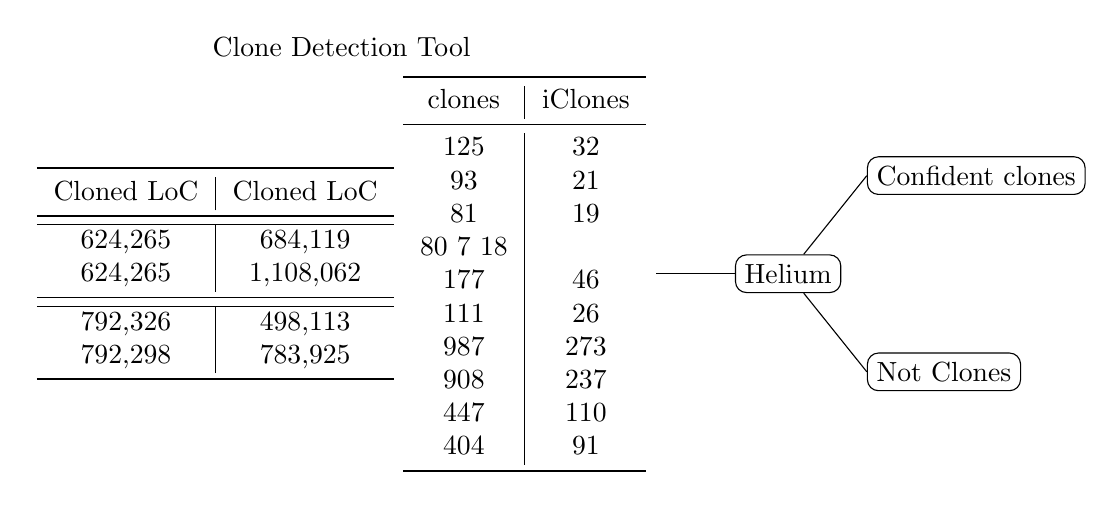
\begin{tikzpicture}

    % \matrix[] (whole) {
    %     \matrix[] (inner) {
    %       \node {Hello};&
    %       \node {World};\\
    %     };&
    %   \node {Delta Debugging};\\
    %   \node {IDE};&
    %   \node {Bug Signature};\\
    % };

    \node (tool) ["Clone Detection Tool"] {
      \begin{tabular}{c | c}
        \toprule
        Cloned LoC & Cloned LoC\\
        \midrule\hline
        624,265 & 684,119\\
        624,265 & 1,108,062\\
        \midrule\hline
        792,326 & 498,113\\
        792,298 & 783,925\\
        \bottomrule
      \end{tabular}

      \begin{tabular}{c|c}
        \toprule
        clones & iClones \\
        \midrule
        125& 32\\
        93& 21\\
        81 & 19\\
        80 7 18\\
        177 & 46\\
        111 & 26\\
        987 & 273\\
        908 & 237\\
        447 & 110\\
        404 & 91\\
        \bottomrule
      \end{tabular}
    };
    \node (helium) [draw, rounded corners, right=of tool] {Helium};
    \node (conf-clone) [draw, rounded corners,
      right=of helium.north, shift={(0,1)}] {Confident clones};
    \node (not-clone) [draw, rounded corners,
      right=of helium.south, shift={(0,-1)}] {Not Clones};

    \draw (tool) -- (helium);
    \draw (helium) -- (conf-clone.west);
    \draw (helium) -- (not-clone.west);
    

  \end{tikzpicture}
\end{figure*}

\begin{figure*}
  \centering
  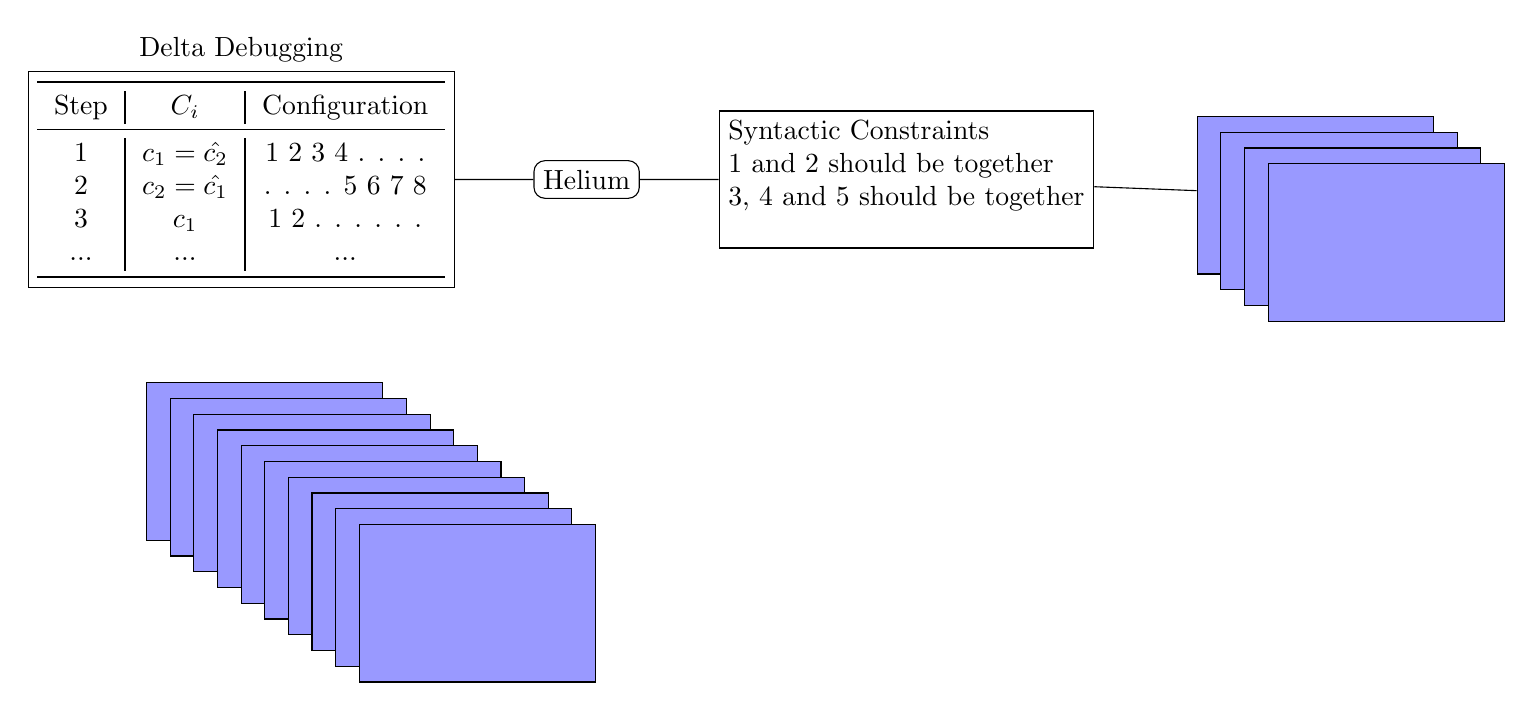
\begin{tikzpicture}
    \node (delta) [draw, "Delta Debugging"] {
      % # a table
      \begin{tabular}{c | c | c}
        
        \toprule
        Step & $C_i$ & Configuration \\
        \midrule
        1 & $c_1 = \hat{c_2}$ & 1 2 3 4 . . . .\\
        2 & $c_2 = \hat{c_1}$ & . . . . 5 6 7 8\\
        3 & $c_1$ &             1 2 . . . . . .\\
        ... & ... & ... \\
        \bottomrule

      \end{tabular}
      % # some visualization
      % \node [draw,
      %   % minimum width=2.2cm,minimum height=2.5cm
      %   % minimum width=3cm, minimum height=3cm
      %   ]{Hello World};

      % \node (innnn) {Hello};
      
    };
    \begin{scope}[every node/.style=draw, minimum width=3cm, minimum height=2cm]
      \foreach \x in {1, 2, 3, 4, 5, 6, 7, 8, 9, 10}
      \node (in-\x) [below=of delta, fill=blue!40, shift={(\x * 0.3 cm, - \x * 0.2 cm)}] {};
    \end{scope}
    
    \node (helium) [draw, rounded corners, right=of delta] {Helium};
    \node (constraint) [draw, right=of helium, align=left] {
      Syntactic Constraints\\
      1 and 2 should be together\\
      3, 4 and 5 should be together\\
    };
    % \node (output) [draw, right=of constraint] {Output};

    \begin{scope}[every node/.style=draw, minimum width=3cm, minimum height=2cm]
      \foreach \x in {1, 2, 3, 4}
      \node (output-\x) [right=of constraint, fill=blue!40, shift={(\x * 0.3 cm, - \x * 0.2 cm)}] {};
    \end{scope}
    

    \draw (delta) -- (helium) -- (constraint) -- (output-1);

    
  \end{tikzpicture}

\end{figure*}

\begin{figure*}
  \centering
  \begin{tikzpicture}
    \node (ide) [draw, minimum width=10cm, minimum height=6cm, align=left] {
      \begin{lstlisting}[style=base]
while (var < 100) {
  if (var > 5) {
    sum += var / 2;
    var += 2;
  } @else@
    @sum += var;@
  var++;
}
\end{lstlisting}
      IDE\\
      Menu:\\
      - View AST/CFG\\
      - Show Patch\\
      - Generate Program\\
      - Run Test\\
      - Analyze\\
    };
    % IDE should have menu
    % IDE should support selection of nodes
    % IDE should output something
    \node (ast) [draw, rounded corners, anchor=north, right=of ide.north east,
      every label quotes/.style={below,white,
            anchor=west,font=\bfseries\scriptsize, shift={(-1em,-0.5em)}}
      ] {
      \begin{forest}
        [$ifstmt$,
          [\texttt{if}, "6"][\texttt{(}, "7"]
          [$expr_2$,
            [\texttt{var>5}, "8"]]
          [\texttt{)}, "9"]
          [$stmt_2$,
            [$compstmt_2$,
              [\texttt{\{}, "10"]
              [$stmt_3$,
                [\texttt{sum+=var/2;}, "11"]]
              [$stmt_4$,
                [\texttt{var += 2;}, "12"]]
              [\texttt{\}}, "13"]]]
          [\color{blue}\texttt{else}, "14"]
          [$stmt_5$,
            [\color{blue}\texttt{sum+=var;}, "15"]]]
  \end{forest}
      };
    \node (patch) [draw, rounded corners, below=of ast, "Patch"] {
            \begin{lstlisting}[style=graycode]
while (var < 100) {
  @if (var > 5) {@
    sum += var / 2;
    var += 2;
  @}@ else
    sum += var;
  var++;
}
\end{lstlisting}
      };
      \node (gen) [draw, rounded corners, below=of patch] {
\begin{lstlisting}[]
int var, sum;
input(var);
input(sum);
if (var > 5) {
} else
  sum += var;
output(var);
output(sum);
\end{lstlisting}
      };
      \node (test) [draw, rounded corners, below=of gen] {
        % test input and output
        \begin{tabular}{c | c | c | c}
          \toprule
          $var_{in}$ & $sum_{in}$ & $var_{out}$ & $sum_{out}$\\
          \midrule\hline
          1 & 2 & 1 & 3\\
          10 & -3 & 10 & -3\\
          .. & .. & .. & ..\\
          \bottomrule
        \end{tabular}
      };

      \node (result) [draw, below=of test, align=left] {
        Transfer Function:\\
        $var_{out} = var_{in}$\\
        % $sum_{out} = sum_{in} + var_{in}$\\

        % $\begin{aligned}
        %   a + b
        % \end{aligned}$

        $\begin{aligned}
          sum_{out} =
          \begin{cases}
            sum_{in} & var_{in} > 5\\
            sum_{in} + var_{in} & otherwise\\
          \end{cases}
        \end{aligned}$
      };


    
    
  \end{tikzpicture}

\end{figure*}


\begin{figure*}
  \centering
  \begin{tikzpicture}
    % Bug Signature

    \node (orig) [draw] {
      \begin{lstlisting}
  static boolean 
  parse_time (const struct parser_table* entry,
              char *argv[], int *arg_ptr)
  {
    struct predicate *our_pred;
    struct time_val tval;
    enum comparison_type comp;
    const char *timearg;
    const char *errmsg = "arithmetic overflow ...";
    time_t origin;
    if (!collect_arg(argv, arg_ptr, &timearg))
      return false;
    origin = options.cur_day_start;
    if (get_comp_type(&timearg, &comp))
      {
        if (COMP_LT == tval.kind)      
          {
            uintmax_t expected = origin + (DAYSECS-1);
            origin += (DAYSECS-1);
            if (origin != expected)
              {
                error(1, 0,
                      _("arithmetic overflow ..."));
              }
          }
      }
    if (!get_relative_timestamp(timearg, &tval, origin,
                                DAYSECS, errmsg))
      return false;
    // ...
  }
\end{lstlisting}
    };

    \node (sig) [draw, right=of orig.north east, anchor=north west] {
\begin{lstlisting}
  static boolean 
  parse_time (char *argv[], int *arg_ptr)
  {
    enum comparison_type comp;
    const char *timearg;
    if (get_comp_type(&timearg, &comp)) {}
    if (!get_relative_timestamp(timearg, &tval, origin,
                                DAYSECS, errmsg))
      return false;
  }
\end{lstlisting}      
    };
    \node (transfer) [draw, below=of sig, align=left] {
      Failure condition:\\
      $\quad orig\_timearg = timearg$\\
      Transfer function:\\
      $\quad orig\_timearg\_out = arg\_ptr + 1$\\
      $\quad timearg = arg\_ptr + 1$\\
      Precondition: $null$\\
    };

  \end{tikzpicture}
\end{figure*}








\end{document}
